%Fiber Optik (Arsitektur Komputer)
%Kelas : D4 TI 1B
%Khadijah Hasanah Putri Harahap 1174022
%Liyana Majdah Rahma 1174039
%Luthfi Muhammad Nabil 1174035
%Nisrina Aulia Firdaus 1174098
%Salwaa Tania 1174047
%Septia Rahayu 1174044
%Diana Satima Gistivani 1154018

\section{Fiber Optic}
\begin{flushleft}
Fiber Optic merupakan sebuah kabel tembus pandang berbahan kaca atau plastik yang halus dan kecil yang digunakan untuk mentransmisikan sinyal cahaya dari satu tempat ke tempat lain, Sumber cahaya dari Fiber Optic biasanya menggunakan cahaya Laser atau LED. Ukuran diameter dari kabel ini kurang lebih sekitar 125 mikrometer atau sekitar 1/8 mm. Kabel Fiber Optic sendiri biasa dipakai dalam kepentingan Jaringan telepon atau Koneksi Internet.
\end{flushleft}
\begin{flushleft}
Gelombang cahaya pada kabel Fiber Optic dipantulkan dari satu ujung ke ujung yang lain tanpa menggunakan perantara apapun, radius dari pantulan cahaya Fiber Optic bisa mencapai 50 Kilometer sedangkan jika memakai perantara seperti repeater dapat mencapai 100 Kilometer. kabel Fiber Optic memiliki daya pantul cahaya yang sangat tinggi sehingga membuat cahaya pada kabel tidak mudah meredup atau melemah dibagian tengah kabel. 
\end{flushleft}
\section{Sejarah Fiber Optic}
\begin{flushleft}
Kabel Fiber Optic mulai dibuat dan dikembangkan pada tahun 1970, saat Ilmuwan dari Corning Glass Works yaitu Donald Keck, Peter Schultz, dan Robert Maurer melaporkan penemuan Fiber Optic yang memenuhi syarat yang ditentukan oleh Kao dan Hockham. Mereka dapat mengurangi kerugian cahaya sampai kurang dari 20 decibels per kilometer menggunakan Kaca murni yang dibuat terdiri dari gabungan silika. Dilanjutkan pada tahun 1972, tim ini menemukan Kaca yang mampu mengurangi kerugian cahaya sampai hanya 4 decibels per kilometer. Pada tahun 1970, Morton Panish dan Izuo Hayashi dari Bell Laboratories mendemonstrasikan laser semikonduktor yang dapat dioperasikan pada temperatur ruang. Dengan adanya penemuan dari kedua tim inilah Kabel Fiber Optik mulai berkembang.
\end{flushleft}
\begin{flushleft}
Pada tahun 1977 Perusahaan telepon mulai menggunakan Fiber Optic dengan mengganti sistem kawat tembaga menjadi jalur Fiber Optic. Perusahaan telepon sendiri menggunakan Fiber Optic diseluruh sistem mereka sebagai sistem komunikasi jarak jauh antar kota. Dengan adanya pemakaian yang meledak membuat Industri Fiber Optic semakin mengalami keuntungan. Pada tahun 1980, sebuah perusahaan AT\&T membuka jaringan Fiber Optic yang menghubungkan kota antara Boston dan Washington D.C. di Amerika. Perusahaan elektronik sendiri mulai mencoba memainkan peranan dalam mendalami riset Fiber Optic.
\end{flushleft}
\begin{flushleft}
Fiber Optic mulai bersifat lebih mudah dikembangkan dan lebih efisien penggunaannya dari masa ke masa, seperti halnya pada tahun 1987 David Payne dari Universitas Southampton yang mengenalkan optical amplifiers yang dicampur oleh elemen erbium yang dapat menaikkan sinyal cahaya tanpa harus dikonversikan ke dalam energi listrik terlebih dahulu juga pada tahun 1991 yaitu Emmanuel Desurvire dan David Payne yang mengintegrasikan kabel Fiber Optic dengan Optical Amplifiers yang membuat informasi sampai 100 kali lebih cepat daripada kabel dengan penguat elektronik.
\end{flushleft}
\begin{flushleft}
Penggunaan Kabel Fiber Optic mulai sangat efektif diantaranya dengan munculnya sebuah kabel jenis TPC-5 yang merupakan kabel Fiber Optic yang menggunakan penguat optik. Kabel ini sudah menghubungkan antara negara - negara yang sudah bekerjasama, mulai dari San Luis Obispo, California, ke Guam, Hawaii, dan Miyazaki dan kabel ini dapat menangani sekitar 320.000 panggilan telepon. dengan berkembangnya kabel Fiber Optic membuat seluruh dunia dapat terhubung dengan mudah.Munculnya Link Around the Globe membuat jaringan kabel Fiber Optic terpanjang dan terluas di seluruh dunia yang telah menyediakan infrastruktur untuk generasi internet terbaru.
\end{flushleft}
\section{Karateristik Fiber Optic}
\begin{flushleft}
\begin{figure}[ht]
\centerline{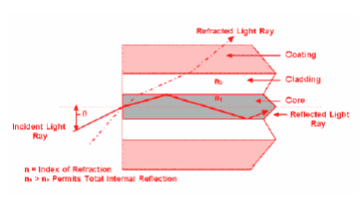
\includegraphics[width=0.6\textwidth]{figures/skemafiber.png}}
\caption{Skema dari Kabel Fiber Optic}
\label{Skema Fiber Optic_03}
\end{figure}
Fiber Optic memberikan dampak yang besar dalam dunia pengiriman sebuah informasi, mulai dari koneksi lokal sampai koneksi antar benua. Fiber optic sendiri merupakan suatu media pengiriman yang sangat pesat perkembangannya. Data yang dikirimkan pada kabel Fiber Optic sendiri berupa analog dan digital. Sistematis pengiriman data berasal dari listrik yang kemudian diubah ke optic oleh sumber cahaya berupa cahaya LED. Seperti pada gambar \ref{Skema Fiber Optic_03}, Kabel Fiber Optic memiliki beberapa Struktur data. Struktur data dari Fiber Optic diantaranya sebagai berikut : 
\begin{enumerate}
\item Core (Inti)\\ Berfungsi untuk menuntukan cahaya yang merambat dari ujung satu ke ujung lainnya. Core sendiri memiliki beberapa ciri - ciri diantaranya : \\ 
	\begin{itemize}
	\item Terbuat dari kuarsa yang berkualitas tinggi
	\item Merupakan dari bagian Fiber Optic
	\end{itemize}
\item Cladding (Lapisan)\\ Berfungsi untuk memantulkan cahaya agar dapat merambat ke ujung satunya. Cladding memiliki beberapa ciri - ciri diantaranya : \\
	\begin{itemize}
	\item Terbuat dari kaca dengan index bias yang lebih rendah dari Core (Inti).
	\item Hubungan antara Cladding dan Core mempengaruhi perambatan cahaya pada core.
	\end{itemize}
\item Coating (Pelindung) \\ Berfungsi sebagai pelindung kabel. Coating memiliki beberapa ciri - ciri diantaranya : \\
	\begin{itemize}
	\item Memiliki bahan dari plastik.
	\item Berfungsi untuk melindungi Fiber Optic dari segala kerusakan.
	\end{itemize}
\end{enumerate}
\end{flushleft}
\begin{flushleft}
Indeks bias pada Core harus lebih besar dari indesk bias pada Cladding. Bahan dari Core sendiri tidak harus terbuat dari bahan yang sejenis dengan Cladding melainkan bisa dibuat dengan menggunakan bahan selembar senar transparan yang berfungsi sebagai core dan Cladding udara dan lain sebagainya. Pada bidang komunikasi Optik, bahan Fiber Optic dibuat menggunakan bahan silica yang murni pada core maupun cladding. Untuk membedakan indeks bias core dan cladding, bahan silica murni diberi campuran yang memiliki kadar berbeda untuk setiap core dan cladding. Bentuk pemampang kabel Fiber Optic yang berbentuk lingkaran ukuran diameternya sekitar 125 mikrometer atau sekitar 1/8 mm.
\begin{figure}[ht]
\centerline{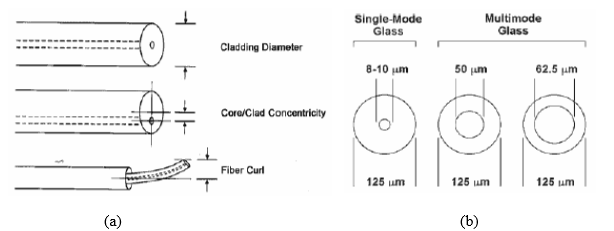
\includegraphics[width=1\textwidth]{figures/sizeanddiameter.png}}
\caption{(a). Diameter Cladding, Core, dan Fiber Curl  (b). Ukuran Fiber Optic}
\label{Skema Fiber Optic_01}
\end{figure}
\end{flushleft}
\begin{flushleft}
Bentuk penampang dari core Fiber Optic adalah berbentuk ellips dan berbentuk lingkaran. Tipe kabel yang umum digunakan dalam kebutuhan telekomunikasi dapat dilihat dari ukuran diameter dari Core. Tipe dari kabel tersebut diantaranya mode tunggal (Single mode/mono mode) dan mode jamak (multi mode). Dari kedua kabel tersebut memiliki banyak perbedaan dimana kabel fiber optic single mode lebih mahal dibandingkan kabel fiber optic multi mode, dimana kabel fiber optic single mode lebih efektif dibandingkan dengan kabel fiber optic multi mode. Jika dilihat dari distribusi indeks bias core, kabel fiber optic memiliki beberapa jenis diantaranya : 
\begin{enumerate}
\item Step Index Multimode \\ Merupakan index bias core konstan yang memiliki ukuran diameter 50 mikrometer dan dilapisi oleh cladding yang sangat tipis. jenis ini dapat digunakan untuk transmisi jarak pendek dan data bit rate rendah.
\item Graded Index Multimode \\ Merupakan cahaya yang dapat merambat karena difraksi yang terjadi pada core sehingga cahaya dapat merambat sejajar dengan sumbu serat
\item Step Index Singlemode \\ Memiliki diameter core yang lebih kecil dibandingkan dengan ukuran cladding
\end{enumerate}
\end{flushleft}
\begin{flushleft}
\begin{figure}[ht]
\centerline{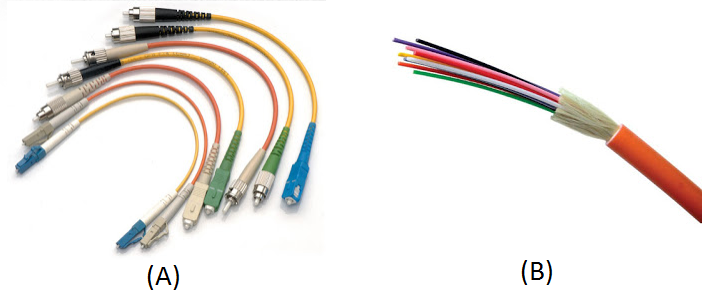
\includegraphics[width=1\textwidth]{figures/patchandmulti.png}}
\caption{(A).Kabel Patchcord  (B). Kabel Multi-Fiber}
\label{Skema Fiber Optic_02}
\end{figure}
Pada pengaplikasian sebuah kabel Fiber Optic dibutuhkannya sebuah kabel yang cocok dan sesuai dengan kondisi pada daerah tersebut. Fiber Optic sendiri memiliki beberapa jenis kabel yang dipakai pada pengaplikasian atau penggunaan sebuah kabel Fiber Optic, beberapa kabel pada umumnya digunakan sebagai perantara untuk pengaplikasian sebuah kabel Fiber Optic diantaranya : 
\begin{itemize}
\item Kabel Patch cords \\ Merupakan kabel Fiber Optic yang digunakan untuk kebutuhan jangka panjang yang terbatas dalam menghubungkan 2 titik jaringan kabel optik. Terdapat 2 tipe patchcord yang digunakan diantaranya menggunakan Single Fiber Optic dan menggunakan Double Fiber Optic. Untuk membedakan penggunaannya, telah dibuatkan standar warna pada kabel tersebut. Penggolongan warna tersebut diantaranya adalah sebagai berikut : \\
	\begin{itemize}
		\item Orange : Multi-mode optical fiber
		\item Aqua : OM3/OM4 10 G laser-optimized 50/125 micrometer multi-mode optical fiber
		\item Violet : OM4 Multi-mode optical fiber
		\item Grey : Outdated color code untuk Multi-mode optical fiber
		\item Yellow : Single-mode optical fiber
		\item Blue : Sebagai penunjuk polarization-maintaning optical fiber
	\end{itemize}
Untuk keperluan terminasi, setiap ujung dari kabel patch cord telah dipasang sebuah konektor. Setiap konektor yang dipasang telah diberi standar warna yang memiliki fungsi yang berbeda - beda, yang digolongkan sebagai berikut : \\
	\begin{itemize}
		\item Blue (Physical Contact (PC), 0) : Pada umumnya digunakan Pada Single Mode
		\item Green (Angle Polished (APC), 8)
		\item Black (Physical Contact(PC), 0)
		\item Grey/Cream (Physical Contact (PC), 0)
		\item White (Physical Contact (PC), 0)
		\item Red : High Power Fiber Optic yang terkadang digunakan untuk menghubungkan External Pump Laser atau Raman Pumps
	\end{itemize}
\end{itemize}
\item Kabel Multi-Fiber \\ Setiap kabel Fiber Optic pada kabel Multi-Fiber menggunakan kode warna untuk membedakan yang satu dengan yang lainnya. Identifikasi yang digunakan menggunakan standar EIA/ TIA-598, "Optical Fiber Cable Color Coding". Dengan menggunakan standar ini setiap unit dapa diidentifikasi menggunakan daftar warna yang ada. Warna - warna yang digunakan beserta kodenya adalah sebagai berikut : \\
\begin{itemize}
\item 1 : Biru - 13 : Biru/Hitam
\item 2 : Oranye - 14 : Oranye/Hitam 
\item 3 : Hijau - 15 : Hijau/Hitam 
\item 4 : Coklat - 16 : Coklat/Hitam 
\item 5 : Abu - Abu : 17 : Abu-Abu/Hitam 
\item 6 : Putih - 18 : Putih/Hitam 
\item 7 : Merah - 19 : Merah/Hitam 
\item 8 : Hitam - 20 : Hitam/Kuning 
\item 9 : Kuning - 21 : Kuning/Hitam 
\item 10 : Ungu - 22 : Ungu/Hitam 
\item 11 : Pink - 23 : Pink/Hitam 
\item 12 : Aqua - 24 : Aqua/Hitam 
\end{itemize}
Selain jenis dan tipe kabel, terdapat juga tipe konektor yang tersedia dalam berbagai bentuk dan kegunaannya tersendiri. Beberapa konektor beserta fungsinya diantaranya adalah sebagai berikut : \\
\begin{enumerate}
\item Fiber Connector (FC) \\ Digunakan pada kabel Single-mode dengan tingkat ketepatan yang sangat tinggi dalam menghubungkan kabel dengan transmitter atau receiver. Fiber Connector menggunakan sistem drat ulir dengan posisi yang dapat diatur sehingga saat dihubungkan ke perangkat lain, level akurasi tidak akan mudah berubah.
\item Subscriber Connector (SC) \\ Digunakan pada kabel Single-mode, dengan sistem cabut-pasang. Konektor ini lebih simpel dan dapat diatur manual dengan akurasi yang baik jika dipasangkan ke perangkat lain.
\item Straight Tip (ST) \\ Bentuknya hampir mirip dengan konektor BNC. Konektor ini paling sering digunakan baik untuk kabel multi mode maupun single mode. Sangat mudah untuk dipasang maupun dicabut.
\item Biconic \\ Salah satu Konektor yang pertama kali muncul dalam komunikasi fiber optic. Pada saat ini konektor tersebut jarang sekali digunakan.
\item D4 \\ Konektor ini hampir sama persis dengan FC hanya saja beda dalam ukuran. Perbedaan pada ukuran sekitar 2mm pada bagian ferrule.
\item SMA \\ Konektor ini merupakan versi lama dari konektor ST yang keduanya memiliki sebuah penutup dan pelindung. Namun dengan berkembangnya konektor ST, Konektor SMA sudah tidak dipakai lagi.
\item E200
\end{enumerate}
\end{flushleft}
\section{Keunggulan Fiber Optic}
\begin{flushleft}
Dengan teknologi Fiber Optic saat ini, Fiber Optic memiliki beragam kelebihan diantaranya : \\
\begin{enumerate}
\item Redaman Transmisi yang kecil \\ Fiber Optic memiliki tingkat redaman transmisi yang dibilang relatif kecil dibanding dengan transmisi lainnya. Yang berarti Fiber Optic sangat sesuai untuk digunakan pada komunikasi jarak jauh, sebab cukup dengan membutuhkan repeater yang jumlahnya lebih sedikit.
\item Radius Frekuensi yang cukup luas \\ Fiber optic dapat digunakan dengan kecepatan yang tinggi hingga mencapai beberapa Gigabit/detik. Dengan begitu sistem ini dapat digunakan untuk membawa sinyal informasi dalam jumlah besar hanya dalam satu buah Fiber Optic yang halus.
\item Ukuran kecil dan ringan \\ Dengan ukuran yang kecil memudahkan pemasangan dan pengangkutan di berbagai lokasi. Misalkan dapat dipasang pada kabel yang sudah tidak terpakai dan memasangkan kabel Fiber Optic ke shield pada kabel lama.
\item Tidak ada gangguan \\ Sistem Transmisi Fiber Optic menggunakan sinar atau laser sebagai gelombang pembawa yang mengakibatkan bebas dari cross talk yang terjadi pada kabel biasa. Atau bisa dibilang kualitas transmisi yang dihasilkan lebih baik dibanding trasmisi dengan kabel. Dengan tidak terjadinnya gangguan akan diutamakan pemasangan kabel Fiber Optic dipasang pada jaringan tenaga listrik tegangan tinggi tanpa khawati akan adanya gangguan yang dipengaruhi oleh tegangan tinggi.
\item Adanya isolasi antara pengirim dan penerima
\item Tidak ada ground loop
\item Tidak memungkinkan terjadinya hubungan api pada saat terputusnya Kabel Fiber Optic. Dengan demikian sangat aman dipasang pada tempat yang mudah terbakar
\end{enumerate}
\end{flushleft}
\section{Rangkuman}
\begin{flushleft}
Fiber Optic merupakan sebuah kabel berbahan kaca yang digunakan untuk mentransmit data berbasis cahaya yang dikirim dari satu ujung ke ujung kabel yang lain. Ukuran normal dari kabel tersebut adalah 125 mikro meter pada diameter. Radius pada kabel fiber optic mampu mencapai 50 Kilometer tanpa menggunakan Repeater. Pembuatan kabel fiber optic dimulai pada tahun 1970 dimana telah ditemukannya pengurangan kerugian cahaya dan laser semikonduktor dan mulai meledak penggunaanya pada tahun 1991. Kabel Fiber Optic memiliki struktur data diantaranya bagian Core, Cladding, dan Coating. Keunggulan dari kabel fiber optic sendiri sangat beragam diantaranya Redaman Transmisi yang kecil sampai Tidak memungkinkan adanya hubungan api saat terputusnya kabel. Dengan hal ini membuat sebuah Kabel Fiber Optic bisa lebih unggul dalam banyak kondisi. 
\end{flushleft}
\cite{nilsson1992preterminated}
\cite{wahyudi2010mengenal}